\documentclass{article}

\usepackage{graphicx}
\usepackage{tikz}
\usepackage{tikzsymbols}
\usetikzlibrary{calc,patterns,shapes.geometric}
\pagestyle{empty}
\usepackage[margin=0pt]{geometry}
\geometry{papersize={14in,12in}}

\def\centerarc[#1](#2)(#3:#4:#5){\draw[#1] ($(#2)+({#5*cos(#3)},{#5*sin(#3)})$) arc (#3:#4:#5);}

\begin{document}
	\begin{figure}
		\centering
		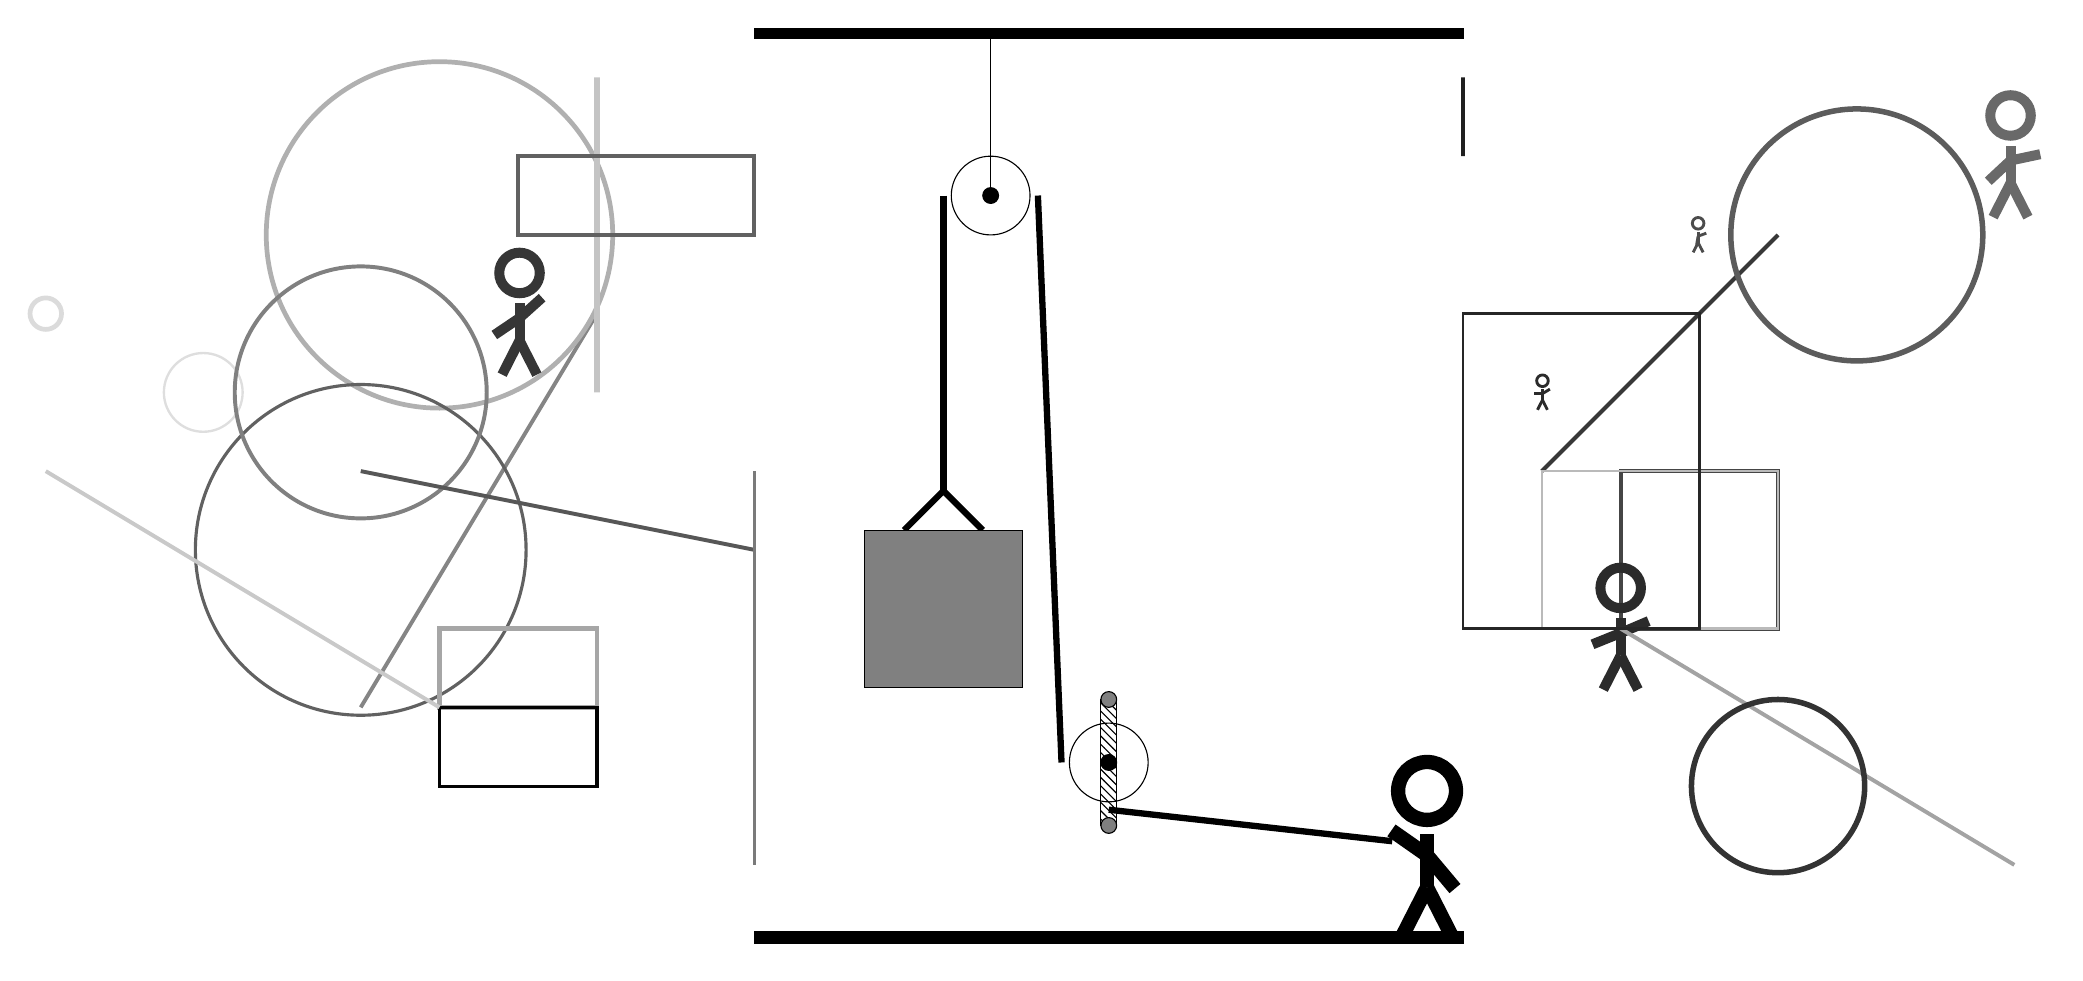
\begin{tikzpicture}
			%%%%% START %%%%%
			
			\draw[fill=black] (-2, 11.5) rectangle (7, 11.625);
			
			\draw[line width=0.5mm, color=black!73] (9, 6) rectangle (11, 4);
			
			\draw [line width=0.6mm, color=black!14](-11, 8) circle (0.2);
			\draw[line width=0.5mm, color=black!48](-7, 3) -- (-4, 8);
			\draw[line width=0.5mm, color=black!78](8, 6) -- (11, 9);
			\draw [line width=0.6mm, color=black!31](-6, 9) circle (2.2);
			\draw [line width=0.4mm, color=black!62](-7, 5) circle (2.1);
			\node[line width=0.4mm, color=black!83] at (9, 4) {\Strichmaxerl[7][22][23]};
			\draw[line width=0.7mm, color=black!23] (-4, 11) rectangle (-4, 7);
			\draw[line width=0.6mm, color=black!35] (-4, 4) rectangle (-6, 3);
			
			\draw[line width=0.5mm, color=black!36](9, 4) -- (14, 1);
			\draw [line width=0.3mm, color=black!13](-9, 7) circle (0.5);
			
			\node[line width=0.5mm, color=black!59] at (14, 10) {\Strichmaxerl[7][43][12]};
			\node[line width=0.3mm, color=black!79] at (-5, 8) {\Strichmaxerl[7][34][42]};
			
			\node[line width=0.5mm, color=black!83] at (8, 7) {\Strichmaxerl[2][0][31]};
			\draw [line width=0.5mm, color=black!50](-7, 7) circle (1.6);
			\draw[line width=0.4mm, color=black!99] (-4, 3) rectangle (-6, 2);
			\draw [line width=0.7mm, color=black!64](12, 9) circle (1.6);
			\draw[line width=0.6mm, color=black!88] (7, 11) rectangle (7, 10);
			\draw[line width=0.5mm, color=black!21](-6, 3) -- (-11, 6);
			\draw[line width=0.5mm, color=black!66](-7, 6) -- (-2, 5);
			\node[line width=0.3mm, color=black!70] at (10, 9) {\Strichmaxerl[2][80][20]};
			
			\draw[line width=0.5mm, color=black!62] (-2, 10) rectangle (-5, 9);
			\draw[line width=0.3mm, color=black!27] (8, 4) rectangle (11, 6);
			\draw[line width=0.3mm, color=black!85] (7, 8) rectangle (10, 4);
			\draw[line width=0.4mm, color=black!52] (-2, 6) rectangle (-2, 1);
			
			\draw [line width=0.7mm, color=black!80](11, 2) circle (1.1);
			
			\draw (1, 9.5) circle (0.5);
			\draw[fill=black] (1, 9.5) circle (0.1);
			\draw (1, 11.5) -- (1, 9.5);
			
			\draw[fill=white](2.5, 2.3) circle (0.5);
			\draw[fill=black] (2.5, 2.3) circle (0.1);
			\draw[pattern=north west lines, pattern color=black] (2.4, 3.1) rectangle (2.6, 1.5);
			\draw[fill=black!50] (2.5, 3.1) circle (0.1);
			\draw[fill=black!50] (2.5, 1.5) circle (0.1);
			
			\draw[line width=0.8mm] (-0.1, 5.25) -- (0.4, 5.75) -- (0.9, 5.25);
			\draw[fill=black!50] (-0.6, 5.25) rectangle (1.4, 3.25);
			
			\draw[line width=0.8mm] (0.4, 9.5) -- (0.4, 5.75);
			\centerarc[line width=0.8mm](1, 9.5)(0:180:0.6);
			\draw[line width=0.8mm](1.6, 9.5) -- (1.9, 2.3);
			\centerarc[line width=0.8mm](2.5, 2.3)(180:270:0.6);
			\draw[line width=0.8mm](2.5, 1.7) -- (6.1, 1.3);
			
			\node at (6.5, 1.2) {\Strichmaxerl[10][-35][-50]};
			
			\draw[fill=black] (-2, 0) rectangle (7, 0.15);
			
			%%%%% END %%%%%
		\end{tikzpicture}
	\end{figure}	
\end{document}